% Created 2017-02-21 Tue 15:37
% Intended LaTeX compiler: pdflatex
\documentclass[10pt,aspectratio=1610]{beamer}
\usepackage[utf8]{inputenc}
\usepackage[T1]{fontenc}
\usepackage{graphicx}
\usepackage{grffile}
\usepackage{longtable}
\usepackage{wrapfig}
\usepackage{rotating}
\usepackage[normalem]{ulem}
\usepackage{amsmath}
\usepackage{textcomp}
\usepackage{amssymb}
\usepackage{capt-of}
\usepackage{hyperref}
\usepackage[english]{babel}\usepackage{etex}
\usepackage{tikz}\usepackage{amsmath}\usepackage[T1]{fontenc}\usepackage{lmodern}%\usepackage{arev}
\usepackage{booktabs}\usepackage[citestyle=alphabetic,bibstyle=authortitle]{biblatex}
\usepackage{pgfplots,pgfplotstable}\usetikzlibrary{pgfplots.groupplots}\usepackage[babel=true,kerning=true]{microtype}\usepackage{smartdiagram}
\addbibresource{intro.bib}
\usetikzlibrary{mindmap,trees,shapes,arrows,spy,3d,decorations.pathmorphing,pgfplots.statistics,pgfplots.dateplot}
\definecolor{c1}{rgb}{0,0,0.562}
\definecolor{c2}{rgb}{0,0,0.875}
\definecolor{c3}{rgb}{0,0.25,1}
\definecolor{c4}{rgb}{0,0.625,1}
\definecolor{c5}{rgb}{0,1,1}
\definecolor{c6}{rgb}{0.375,1,0.625}
\definecolor{c7}{rgb}{0.688,1,0.312}
\definecolor{c8}{rgb}{1,0.938,0}
\definecolor{c9}{rgb}{1,0.562,0}
\definecolor{c10}{rgb}{1,0.188,0}
\definecolor{c11}{rgb}{0.812,0,0}
\definecolor{c12}{rgb}{0.5,0,0}
\usetheme{DarkConsole}
\author{Mathieu Fauvel}
\date{\textit{[2017-04-26 Wed 08:30]--[2017-04-26 Wed 10:00]}}
\title{Introduction to hyperspectral remote sensing imagery}
\subtitle{GRSS Summer School}
\institute{UMR Dynafor}
\AtBeginSection[]{\begin{frame}<beamer>\frametitle{Outline}\tableofcontents[currentsection]\end{frame}}
\AtBeginSubsection[]{\begin{frame}<beamer>\frametitle{Outline}\tableofcontents[currentsubsection]\end{frame}}
\setbeamercovered{again covered={\opaqueness<1->{25}}}
\usefonttheme[onlymath]{serif}
\begin{document}

\maketitle
\begin{frame}{Outline}
\tableofcontents
\end{frame}

\begin{frame}[label={sec:orgb07ce86}]{Mathieu Fauvel}
\begin{center}
\begin{tabular}{ccc}
  \includegraphics[width=0.3\linewidth]{figures/logo-INRA-transp.png}
  &\includegraphics[width=0.3\linewidth]{figures/logoUT.pdf}
  &\includegraphics[width=0.3\linewidth]{figures/inp-ensat.jpg}
\end{tabular}
\end{center}
\begin{itemize}
\item Associate professor at  \href{http://ensat.fr/}{ENSAT} - \href{http://inp-toulouse.fr/}{INP Toulouse} \& \href{http://www.univ-toulouse.fr/}{University of Toulouse}
\item Director of the Engineering and Digital Sciences Department at the National Institute of Agronomy of Toulouse (ENSAT).
\item Associated to the \href{http://dynafor.toulouse.inra.fr/}{DYNAFOR} lab
\item IEEE GRSS:
\begin{itemize}
\item Senior Member
\item Member of the \emph{GRSS Chapter Committee}
\item IEEE JSTARS Associated Editor
\end{itemize}
\end{itemize}
\end{frame}
\section{Introduction}
\label{sec:orgdca8443}
\begin{frame}[label={sec:orge91be9e}]{Remote sensing}
\begin{columns}
\begin{column}{0.5\columnwidth}
[[\begin{center}
\includegraphics[width=\linewidth]{./figures/remote_sensing_acquisition.png}
\end{center}]
\emph{Image taken from \cite{974727}}.
\end{column}
\begin{column}{0.5\columnwidth}
\begin{itemize}
\item Remote   sensing  provides   information   about  landscapes.
\item This information is carried out by the \emph{electromagnetic energy} and is
usually formated in terms of \emph{digital image data}.
\item This information can be used
\begin{itemize}
\item To \emph{update} and to \emph{supervise} landscapes in known areas,
\item To \emph{get prior} information about landscapes of unknown areas.
\end{itemize}
\end{itemize}
\end{column}
\end{columns}
\end{frame}
\begin{frame}[fragile,label={sec:org21a1114}]{Fields of application}
\tikzset{grow cyclic list/.code={%
  \def\tikzgrowthpositions{{#1}}%
  \foreach \n [count=\i,remember=\i]in {#1}{}%
  \let\tikzgrowthpositionscount=\i%
  \tikzset{growth function=\tikzgrowcycliclist}}}
\def\tikzgrowcycliclist{%
  \pgftransformshift{%
    \pgfpointpolar{\tikzgrowthpositions[mod(\the\tikznumberofcurrentchild-1,\tikzgrowthpositionscount)]}%
      {\the\tikzleveldistance}}}
\begin{center}
\resizebox{0.75\textwidth}{!}{
  \begin{tikzpicture}[<->,mindmap,every node/.append style={concept,execute at begin node=\hskip0pt},grow cyclic,
    level 1/.append style={level distance=4.25cm,sibling angle=72,every child/.append style={concept color=black,text=white,font=\bfseries}},%
    level 2/.append style={level distance=3cm,every child/.append style={concept color=gray!75,text=black,font=\small},sibling angle=45},%sibling angle=45
    root concept/.append style={concept color=black, fill=white, line width=1ex, text=black,font=\large},
    ]
    \node [root concept] (hyper) {\textsc{Hyperspectral}\\ \textsc{Images}}[grow cyclic list={45,-25,-150,115,-100,164}] 
    child { node  (lm) {Land\\ management}[clockwise from=90]
      child {node (biomass) {Biomass}}
      child {node (biodiversity) {Biodiversity}}
      child {node (lulc) {Land use/land cover}}
      child {node (cd) {Change detection}}
    }
    child {node (geology) {Geology}[clockwise from=15]
      child {node (det) {Mineral detection}}
      child {node (soil) {Soil composition}}
    }
    child {node (pa) {Precision agriculture}[clockwise from=-120]
      child {node (ns) {Nutrient stress}}
      child {node (ws) {Water stress}}
      child {node (pp) {Plant pathogens}}
    }
    child {node (hydrology) {Hydrology}[clockwise from=180]
      child {node (wq) {Water quality}}
      child {node (coast) {Costal zone}}
    }
    child {node (military) {Military}[clockwise from=0]
      child {node (target) {Target detection}}
    }
    child[level distance= 6cm] {node (urban) {Urban}[clockwise from=180]
      child {node (target) {Polution}}
      child {node (target) {Vegation mapping}}
    };
    \end{tikzpicture}}
\end{center}
\end{frame}
\begin{frame}[label={sec:org1e09f30}]{Hekla Volcano, Iceland}
\begin{columns}
\begin{column}{0.45\columnwidth}
\begin{center}
\includegraphics[width=\linewidth]{figures/hekla_original.jpg}
\end{center}
\end{column}
\begin{column}{0.45\columnwidth}
\begin{center}
\includegraphics[width=\linewidth]{figures/hekla_classif.jpg}
\end{center}
\end{column}
\end{columns}

\begin{block}{Classes}
\textcolor{c1}{Lava 1970}, \textcolor{c2}{Lava 1980 I},  \textcolor{c3}{Lava 1980 II},  \textcolor{c4}{Lava 1991 I}, \textcolor{c5}{Lava 1991 II}, \textcolor{c6}{Lava moss cover}, \textcolor{c7}{hyaloclastite formation}, \textcolor{c8}{Tephra lava}, \textcolor{c9}{Rhyolite}, \textcolor{c10}{Scoria}, \textcolor{c11}{Firn-glacier ice}, \textcolor{c12}{Snow}.
\end{block}
\end{frame}

\section{Hyperspectral imagery}
\label{sec:orgb54ee35}
\subsection{Element of physics}
\label{sec:org5d02ebd}
\begin{frame}[label={sec:orgbfc5539}]{Electromagnetic wave}
\begin{center}
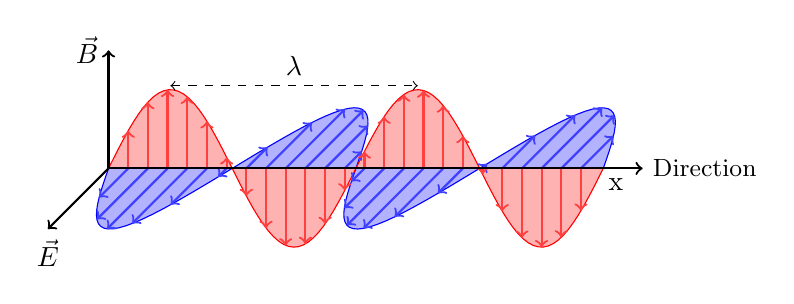
\begin{tikzpicture}[samples=100]
  \filldraw[domain=0:2*pi,color=blue,fill=blue!30] plot (\x,0,{2*sin(\x*2 r)});
  \filldraw[domain=0:2*pi,color=red,fill=red!30] plot (\x,{sin(\x*2 r)},0);
  \foreach \x in {0.25,0.5,...,6}
  {
    \draw[color=blue!75,->,thick] (\x,0,0) -- (\x,0,{2*sin(2*\x r)});
    \draw[color=red!75,->,thick] (\x,0,0) -- (\x,{sin(2*\x r)},0);
  }
  \draw[thick,->] (0,0,0) -- (2*pi+0.5,0,0) node[below, pos=0.95] {x} node[right] {\small Direction};
  \draw[thick,->] (0,0,0) -- (0,1.5,0) node[left] {$\vec{B}$};
  \draw[thick,->] (0,0,0) -- (0,0,2) node[below] {$\vec{E}$};
  \draw[<->,dashed] (pi/4,1.05,0) -- (5*pi/4,1.05,0) node[midway,above] {$\lambda$};
\end{tikzpicture}
\end{center}

\begin{itemize}
\item An electromagnetic wave is a pertubation of the electric and magnetic field which propagates throught space.
\item \(\vec{E}\): Electric field. \(\vec{B}\): Magnetic field.
\item \alert{Wavelength} (\(\lambda\)): \emph{Minimal distance between 2 points of the   space for which \(\vec{E}\) and \(\vec{B}\) recover the same values.}
\end{itemize}
\begin{center}
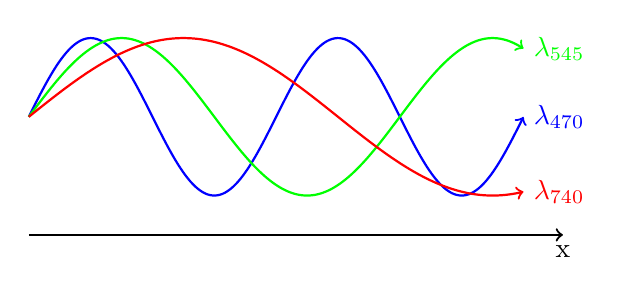
\begin{tikzpicture}[samples=200,domain=0:2*pi]
  \draw[blue,thick,->] plot (\x,{sin(\x*2 r)})node[right] {$\lambda_{470}$};
  \draw[green,thick,->] plot(\x,{sin(\x*2/1.5 r)})node[right] {$\lambda_{545}$};
  \draw[red,thick,->] plot (\x,{sin(\x*2/2.5 r)}) node[right] {$\lambda_{740}$};
  \draw[thick,->] (0,-1.5) -- (2*pi+0.5,-1.5) node[below] {x};
\end{tikzpicture}
\end{center}
\end{frame}
\begin{frame}[label={sec:org615622d}]{Electromagnetic spectrum}
\begin{center}
\includegraphics[angle=-1,width=0.8\linewidth]{./figures/spectralInformation.pdf}
\end{center}

From \cite{manolakis2016hyperspectral}.
\end{frame}
\begin{frame}[label={sec:org202fc96}]{Spectral reflectance}
\alert{Reflectance}: 
\begin{itemize}
\item Capacity of a given surface to reflect the incident light,
\item It is specific to each material.
\end{itemize}

\begin{columns}
\begin{column}{0.4\columnwidth}
\begin{center}
\includegraphics[width=.9\linewidth]{./figures/grss_image.png}
\end{center}
\end{column}
\begin{column}{0.5\columnwidth}
\begin{center}
  \begin{tikzpicture}
    \begin{axis}[small,grid,width=\linewidth,height=0.55\textheight,thick,xmin=410,xmax=995,legend pos=north west,legend style={font=\footnotesize}]
      \addplot[mark=none] table [x=X,y=P1,col sep=comma] {figures/pixels.csv};
      \addplot[mark=none,blue] table [x=X,y=P2,col sep=comma] {figures/pixels.csv};
      \addplot[mark=none,red] table [x=X,y=P3,col sep=comma] {figures/pixels.csv};
      \addplot[mark=none,orange] table [x=X,y=P4,col sep=comma] {figures/pixels.csv};
      \addplot[mark=none,magenta] table [x=X,y=P5,col sep=comma] {figures/pixels.csv};
      \legend{1,2,3,4,5}
    \end{axis}
  \end{tikzpicture}
\end{center}
\end{column}
\end{columns}
\end{frame}
\begin{frame}[label={sec:orgfaa63ef}]{Spectral reflectance curves}
\alert{Spectral reflectance curves or spectral signature}: Radiometric identity card

\begin{center}
\begin{tikzpicture}
\begin{axis}[xmin=0.4,xmax=2.5,ymin=0,ymax=1,grid,xlabel=$\lambda~({\mu}m)$,ylabel=Reflectance,width=0.9\linewidth,height=0.5\linewidth,cycle list name=color list]
  \addplot+[mark=none,thick,smooth] file {figures/oak.txt};
  \pgfplotstableread{figures/grass.txt}\loadedtable
  \addplot+[mark=none,smooth,thick] table[x=wave,y=grass] from \loadedtable;
  \addplot+[mark=none,smooth,thick] table[x=wave,y=drygrass] from \loadedtable;
  \pgfplotstableread{figures/talc.txt}\loadtable
  \addplot+[mark=none,smooth,thick] table[x=wave,y=talc] from \loadtable;
  \legend{Oak,Grass, Dry-Grass, Talc}
\end{axis}
\end{tikzpicture}
\end{center}
\end{frame}
\subsection{Digital remote sensing images}
\label{sec:org7f32dd5}
\begin{frame}[label={sec:org91b30e1}]{Remote sensing images}
\emph{A  remote sensing  image  is a  sampling of  a  spatial, spectral  and
temporel process}.

\begin{center}
\begin{tikzpicture}[spy using outlines={circle, magnification=3, size=1.75cm, connect spies}]
      \visible<1>{\node at (-4,0) {\includegraphics[width=4cm]{figures/46.jpg}};
      \node at (-1.25,-2.5) {\begin{axis}[xmin=407,xmax=985,ymin=0,ymax=1,grid,width=5cm,height=3cm,footnotesize,axis x line=left,axis y line=left]
        \addplot[thick,smooth] file {figures/spectre_full.txt};
      \end{axis}};}
      \visible<2>{\node at (-4,0) {\includegraphics[width=4cm]{figures/46_8.jpg}};
        \draw[very thin] (-6,-2) grid[step = 0.125] (-2,2);        
        \node at (-1.25,-2.5) {\begin{axis}[xmin=407,xmax=985,ymin=0,ymax=1,grid,width=5cm,height=3cm,footnotesize,axis x line=left,axis y line=left]
            \addplot[thick,smooth] file {figures/spectre_8.txt};
          \end{axis}}; 
      } 
      \visible<3-4>{\node at (-4,0) {\includegraphics[width=4cm]{figures/46_8.jpg}};
        \draw[very thin] (-6,-2) grid[step = 0.125] (-2,2);
        \node at (-1.25,-2.5) {\begin{axis}[xmin=407,xmax=985,ymin=0,ymax=1,grid,width=5cm,height=3cm,footnotesize,axis x line=left,axis y line=left]
            \addplot[thick,mark=*,only marks] file {figures/spectre_ss.txt};
          \end{axis}};
      }
      \visible<4>{\draw[->,line width= 1pt] (-6.2,-3.5) -- (5.75,-3.5) node[above] {$t$};
        \foreach \x / \xtext in {-6/January,-5/February,-4/March,-3/April,-2/May,-1/June,0/Jully,1/\textcolor{red}{August},2/September,3/October,4/November,5/December}{
          \fill (\x,-3.5) circle [radius=2pt];
          \node at (\x,-4) {\rotatebox{30}{\footnotesize\xtext}};
        }
      }
      \spy [gray] on (-4.5,1.5) in node [left] at (0.5,1.5);
      \fill[gray] (-4.46,1.53) circle (0.02);
      \fill[white] (4,0) rectangle +(0.04,0.04);
    \end{tikzpicture}
  \end{center}
\end{frame}
\begin{frame}[label={sec:orgceb65f8}]{Characteristics of remote sensing images}
\begin{itemize}
\item Spatial resolution: \emph{Ability to distinguish two closed objects}.
\begin{center}
  \begin{tabular}{cc}
    
\begin{tikzpicture}[thick,scale=0.5,gray]
    \draw (0,0) -- (2,0) -- (2,2) -- (0,2) -- (0,0);    
    \end{tikzpicture}
    &
      
\begin{tikzpicture}[thick,scale=0.5,gray]
        \draw (0,0) -- (2,0) -- (2,2) -- (0,2) -- (0,0);
        \draw (1,0) -- (1,2);
        \draw (0,1) -- (2,1);
      \end{tikzpicture}\\
    2 m/pixel & 1m/pixel
  \end{tabular}
\end{center}
\item Radiometric resolution: \emph{Smallest difference in intensity that the sensor can record}.
\begin{center}
\begin{tabular}{lrr}
\toprule
Coding & Quantification & Exemple: 6.666666\\
\midrule
8 bits & 256 & 7\\
16 bits & 65536 & 6.67\\
\bottomrule
\end{tabular}
\end{center}

\item \uline{Spectral resolution}: \emph{Width of each band of the spectrum that can be collected}.
\begin{center}
\begin{tabular}{{lc}}
\toprule
Image Type & Number of bands\\
\midrule
Panchromatic & 1\\
Multispectral & \textasciitilde{} 10\\
\midrule
Hyperspectral & > 100\\
Ultraspectral & > 100\\
\bottomrule
\end{tabular}
\end{center}
\item Spatial and spectral  resolution are linked: difficult  to have high
spatial \emph{and} spectral resolution at the same time.
\end{itemize}
\end{frame}
\begin{frame}[label={sec:org778179a}]{Multispectral versus hyperspectral}
\begin{center}
\begin{tikzpicture}[]
  \begin{axis}[,xmin=0.4,xmax=2.56,ymin=0,ymax=0.6,grid=both,width=0.9\linewidth,height=0.8\textheight,title=Pleiade versus Hypxim]
    \pgfplotstableread{figures/peuplier_hypxim.txt}\loadedtable
    \addplot+[mark=none,blue,very thick,smooth] table[x=Wavelength,y=A] from \loadedtable;
    \pgfplotstableread{figures/peuplier_pleiades.txt}\loadedtable
    \addplot+[mark=*,very thick,red] table[x=Wavelength,y=A] from \loadedtable;
  \end{axis}
  \end{tikzpicture}
\end{center}
\end{frame}
\begin{frame}[label={sec:orga8a66c1}]{Hyperspectral sensors}
\begin{center}
  \begin{tikzpicture}
  \begin{semilogxaxis}[grid=both,xlabel= \small Spatial resolution (in meters per pixel),ylabel=\small Number of spectral channels,legend style={cells={anchor=east},legend pos=outer north east,},width=0.9\linewidth,height=0.95\textheight,xmax=1300,ymin=0,ymax=320,every node near coord/.append style={font=\small}]      
    \addplot[color=red,scatter,mark size=3,only marks, nodes near coords*={\mysensor},visualization depends on={value\thisrow{sensor}\as\mysensor}] table[x=spa,y=ns,col sep=comma]{figures/table_sensor_airplaine.csv};
    \addplot[color=blue,scatter,mark size=3,only marks, nodes near coords*={\mysensor},visualization depends on={value\thisrow{sensor}\as\mysensor}] table[x=spa,y=ns,col sep=comma]{figures/table_sensor_satellite.csv};
    \end{semilogxaxis}
  \end{tikzpicture}
\end{center}
\end{frame}
\subsection{Spectral signatures}
\label{sec:orgadfe11b}
\begin{frame}[label={sec:org7622c67}]{Vegetation 1/2}
Healthy vegetation (high photosynthesis)
\begin{itemize}
\item Absorption in \emph{blue} and \emph{red} domain,
\item \emph{Visible} to \emph{near infrared}: increase of the reflectance,
\item \emph{Mid infrared}: depends on the free water in the leafs.
\end{itemize}

\begin{center}
\includegraphics[width=0.5\linewidth]{./figures/spectral_curve_vegetation.jpg}
\end{center}
\end{frame}
\begin{frame}[label={sec:orgf658d98}]{Vegetation 2/2}
\begin{columns}
\begin{column}{0.35\columnwidth}
Factor modifying the reflectance
\begin{itemize}
\item Leaf thickness,
\item Leaf age,
\item Water content,
\item Nitrogen content,
\item Health condition,
\item \ldots{}
\end{itemize}
\end{column}

\begin{column}{0.6\columnwidth}
\begin{center}
\begin{tikzpicture}
\begin{axis}[xmin=0.4,xmax=2.5,ymin=0,ymax=1,grid,xlabel=$\lambda~({\mu}m)$,ylabel=Reflectance,width=\linewidth,cycle list name=color list]
  \pgfplotstableread{figures/grass.txt}\loadedtable
  \addplot+[mark=none,smooth,thick] table[x=wave,y=grass] from \loadedtable;
  \addplot+[mark=none,smooth,thick] table[x=wave,y=drygrass] from \loadedtable;
  \legend{Grass, Dry-Grass}
\end{axis}
\end{tikzpicture}
\end{center}
\end{column}
\end{columns}
\end{frame}
\begin{frame}[label={sec:org459ede6}]{Water}
\begin{center}
  \begin{tikzpicture}
    \begin{axis}[xmin=400,xmax=2500,ymin=0,ymax=0.1,grid,xlabel=$\lambda~({\mu}m)$,ylabel=Reflectance,width=0.9\linewidth,height=0.5\linewidth,cycle list name=color list,/pgf/number format/1000 sep={},/pgf/number format/fixed,]
      \pgfplotstableread[col sep=comma]{figures/water_spectra.csv}\loadedtable
      %% 1
      \addplot+[mark=none,smooth,thick, restrict x to domain=410:1345,forget plot] table[x=wave,y=w1] from \loadedtable;
      \addplot+[mark=none,smooth,thick, restrict x to domain=1500:1810,forget plot] table[x=wave,y=w1] from \loadedtable;
      \addplot+[mark=none,smooth,thick, restrict x to domain=1950:2470] table[x=wave,y=w1] from \loadedtable;

      %% 2
      \addplot+[mark=none,smooth,thick, restrict x to domain=410:1345,forget plot] table[x=wave,y=w2] from \loadedtable;
      \addplot+[mark=none,smooth,thick, restrict x to domain=1500:1810,forget plot] table[x=wave,y=w2] from \loadedtable;
      \addplot+[mark=none,smooth,thick, restrict x to domain=1950:2470] table[x=wave,y=w2] from \loadedtable;

      %% 3
      \addplot+[mark=none,smooth,thick, restrict x to domain=410:1345,forget plot] table[x=wave,y=w3] from \loadedtable;
      \addplot+[mark=none,smooth,thick, restrict x to domain=1500:1810,forget plot] table[x=wave,y=w3] from \loadedtable;
      \addplot+[mark=none,smooth,thick, restrict x to domain=1950:2470] table[x=wave,y=w3] from \loadedtable;

      %% 4
      \addplot+[mark=none,smooth,thick, restrict x to domain=410:1345,forget plot] table[x=wave,y=w4] from \loadedtable;
      \addplot+[mark=none,smooth,thick, restrict x to domain=1500:1810,forget plot] table[x=wave,y=w4] from \loadedtable;
      \addplot+[mark=none,smooth,thick, restrict x to domain=1950:2470] table[x=wave,y=w4] from \loadedtable;

    \end{axis}
  \end{tikzpicture}
\end{center}
\end{frame}
\begin{frame}[label={sec:org058119b}]{Human made materials}
\begin{center}
  \begin{tikzpicture}
    \pgfplotsset{every axis legend/.append style={at={(0.5,1.03)},anchor=south}}
    \begin{axis}[grid=both,width=\linewidth,height=0.5\linewidth,xmin=0.350,xmax=2.400,mark=none,/pgf/number format/1000 sep={},/pgf/number format/fixed,thick,ticklabel style = {font=\footnotesize},legend columns=3,xlabel=$\lambda~({\mu}m)$,ylabel=Reflectance (\%)]
      \addplot[] table[x=Wavelength,y=Black rubber,col sep=comma]{figures/manmade_lib.csv};
      \addplot[red,] table[x=Wavelength,y=Window glass,col sep=comma]{figures/manmade_lib.csv};
      \addplot[blue,] table[x=Wavelength,y=Slate sonte,col sep=comma]{figures/manmade_lib.csv};
      \addplot[yellow,] table[x=Wavelength,y=White marble,col sep=comma]{figures/manmade_lib.csv};
      \addplot[orange,] table[x=Wavelength,y=Fiberglass,col sep=comma]{figures/manmade_lib.csv};
      \addplot[magenta,] table[x=Wavelength,y=Rubberized coating,col sep=comma]{figures/manmade_lib.csv};
      \legend{Black rubber,Window glass,Slate sonte,White marble,Fiberglass,Rubberized coating}
    \end{axis}
  \end{tikzpicture}
\end{center}
\end{frame}
\section{Current challenges in hyperspectral}
\label{sec:orgdf7841b}
\subsection{What is remote sensing made of ?}
\label{sec:orgdc98a75}
\begin{frame}[label={sec:org1626cdb}]{An interdisciplinary field}
\begin{center}
\smartdiagramset{planet color=orange!60,
distance planet-satellite=4cm
}
\smartdiagram[bubble diagram]
{\textsc{Hyperspectral}\\ \textsc{Remote Sensing},Computer \\Science,Signal and Image \\ Processing, Pattern \\Recognition, Physics, Environemental\\ Science}
\end{center}
\end{frame}
\begin{frame}[label={sec:org96e3db2}]{Processing chain}
\smartdiagramset{uniform sequence color=true,
sequence item border color=black,sequence item font size=\small,
sequence item text color=white,sequence item text width=2.75cm
}
\begin{center}
  \smartdiagram[sequence diagram]{
    Acquisition, Transmission, Pre-processing, Information extraction}
\end{center}
\begin{itemize}
\item \uline{Transmission}:
\begin{itemize}
\item Compression.
\end{itemize}
\item \uline{Pre-processing}:
\begin{itemize}
\item Geometric and atmospheric corrections,
\item Data fusion,
\item Feature extraction.
\end{itemize}
\item \uline{Information extraction}:
\begin{itemize}
\item Classification/inversion,
\item Unmixing,
\item Target detection.
\end{itemize}
\end{itemize}
\end{frame}

\begin{frame}[label={sec:orgafbaeb4}]{Hot topics}
\begin{center}
  \begin{tikzpicture}
    \begin{axis}[date coordinates in=x,xtick=data, ybar,title=Number of published papers per year about "hyperspectral remote sensing" (\emph{ISI Web of science}),width=0.9\linewidth,height=0.9\textheight,grid=both,date ZERO=1999-09-01,xmin=1999-09-01,xmax=2016-05-01,xticklabel style={rotate=45},xticklabel={\year},ymin=0,ymax=800]
      \addplot coordinates{
        (2000-01-01,80)
        (2001-01-01,100)
        (2002-01-01,125)
        (2003-01-01,210)
        (2004-01-01,225)
        (2005-01-01,195)
        (2006-01-01,275)
        (2007-01-01,290)
        (2008-01-01,270)
        (2009-01-01,345)
        (2010-01-01,355)
        (2011-01-01,360)
        (2012-01-01,510)
        (2013-01-01,555)
        (2014-01-01,640)
        (2015-01-01,740)
        (2016-01-01,645)};      
    \end{axis}
  \end{tikzpicture}
\end{center}
\end{frame}
\subsection{Current challenges}
\label{sec:org13d552d}
\begin{frame}[label={sec:orgfbea7e2}]{Challenges}
\begin{itemize}
\item \uline{Pattern recognition}:
\begin{itemize}
\item High dimensional data,
\item Spectral variability,
\item Reduce ground-thruth,
\end{itemize}
\item \uline{Computer science}:
\begin{itemize}
\item Large volume of data
\item Real time constraints
\end{itemize}
\item \uline{Thematic application}:
\begin{itemize}
\item Environmental issues
\item Military issues
\item Astrophysical issues
\end{itemize}
\end{itemize}
\end{frame}

\begin{frame}[label={sec:org453ca97}]{Spectral variability}
\begin{center}
  \begin{tikzpicture}
    \begin{axis}[grid=both,width=\linewidth,height=0.5\linewidth,xmin=350,xmax=2400,ymin=0,ymax=0.5,mark=none,/pgf/number format/1000 sep={},/pgf/number format/fixed,thick,ticklabel style = {font=\footnotesize},title=Grasslands measurements]
      %% 1
      \addplot[restrict x to domain=350:1350] table[x=x,y=y1,col sep=comma]{figures/spectralSamples.csv};
      \addplot[restrict x to domain=1410:1810] table[x=x,y=y1,col sep=comma]{figures/spectralSamples.csv};
      \addplot[restrict x to domain=1970:2400] table[x=x,y=y1,col sep=comma]{figures/spectralSamples.csv};
      %% 2
      \addplot[red,restrict x to domain=350:1350] table[x=x,y=y2,col sep=comma]{figures/spectralSamples.csv};
      \addplot[red,restrict x to domain=1410:1810] table[x=x,y=y2,col sep=comma]{figures/spectralSamples.csv};
      \addplot[red,restrict x to domain=1970:2400] table[x=x,y=y2,col sep=comma]{figures/spectralSamples.csv};
      %% 3
      \addplot[blue,restrict x to domain=350:1350] table[x=x,y=y40,col sep=comma]{figures/spectralSamples.csv};
      \addplot[blue,restrict x to domain=1410:1810] table[x=x,y=y40,col sep=comma]{figures/spectralSamples.csv};
      \addplot[blue,restrict x to domain=1970:2400] table[x=x,y=y40,col sep=comma]{figures/spectralSamples.csv};
      %% 4
      \addplot[orange,restrict x to domain=350:1350] table[x=x,y=y36,col sep=comma]{figures/spectralSamples.csv};
      \addplot[orange,restrict x to domain=1410:1810] table[x=x,y=y36,col sep=comma]{figures/spectralSamples.csv};
      \addplot[orange,restrict x to domain=1970:2400] table[x=x,y=y36,col sep=comma]{figures/spectralSamples.csv};
      %% 5
      \addplot[green,restrict x to domain=350:1350] table[x=x,y=y50,col sep=comma]{figures/spectralSamples.csv};
      \addplot[green,restrict x to domain=1410:1810] table[x=x,y=y50,col sep=comma]{figures/spectralSamples.csv};
      \addplot[green,restrict x to domain=1970:2400] table[x=x,y=y50,col sep=comma]{figures/spectralSamples.csv};
      %% 6
      \addplot[yellow,restrict x to domain=350:1350] table[x=x,y=y20,col sep=comma]{figures/spectralSamples.csv};
      \addplot[yellow,restrict x to domain=1410:1810] table[x=x,y=y20,col sep=comma]{figures/spectralSamples.csv};
      \addplot[yellow,restrict x to domain=1970:2400] table[x=x,y=y20,col sep=comma]{figures/spectralSamples.csv};
    \end{axis}
  \end{tikzpicture}
\end{center}
\end{frame}
\subsection{High dimensional data}
\label{sec:org23e0ad6}
\begin{frame}[label={sec:orgdb8c85b}]{Properties of HD spaces 1/3}
\begin{itemize}
\item High number of measurements \(d\) but limited number \(n\) of samples.
\item High dimensional space do not behave as low/moderate dimensional space \cite{661089}:
\begin{itemize}
\item Volume of an hypersphere: \(V_s(d,r)=\frac{\pi^{d/2}}{\Gamma\left(\frac{d}{2}+1\right)}r^d\),
\item Volume of an hypercube: \(V_c(d,r)=(2r)^d\).
\end{itemize}
\end{itemize}
\begin{columns}
\begin{column}{0.45\columnwidth}
\begin{center}
  \begin{tikzpicture}
    \begin{axis}[grid=both,xlabel= \small $d$,ylabel= \(V_{s}(d)\),legend style={cells={anchor=east},legend pos=outer north east,},width=0.85\linewidth,xmin=1,xmax=20,ymin=0,ymax=6]      
    \addplot[mark=*] table[x=d,y=s,col sep=comma]{figures/volHs.csv};
  \end{axis}
  \end{tikzpicture}
\end{center}
\end{column}

\begin{column}{0.45\columnwidth}
\begin{center}
  \begin{tikzpicture}
    \begin{axis}[grid=both,xlabel= \small $d$,ylabel=$V_s(d)/V_c(d)$,legend style={cells={anchor=east},legend pos=outer north east,},width=0.85\linewidth,xmin=1,xmax=20,ymin=0,ymax=1]      
    \addplot[mark=*] table[x=d,y=r,col sep=comma]{figures/volHs.csv};
  \end{axis}
  \end{tikzpicture}
\end{center}
\end{column}
\end{columns}
\end{frame}

\begin{frame}[label={sec:org2675437}]{Properties of HD spaces 2/3}
Consider                                                             a
r.v.      \(\mathbf{x}\sim\mathcal{N}(\mathbf{0},\mathbf{I})\).      The
likelihood of \(t=\|\mathbf{x}\|\) is given by

\begin{eqnarray*}
  f(t)= \frac{ t^{d-1}\exp(-t^2/2)}{2^{(d/2)-1}\Gamma(d/2)}
\end{eqnarray*}
which is maximum for \(t^*=\sqrt{d-1}\) \cite{661089}.

\begin{center}
  \begin{tikzpicture}
    \pgfplotsset{every axis legend/.append style={at={(0.5,1.03)},anchor=south}}
    \begin{axis}[grid=both,width=0.9\linewidth,height=0.35\linewidth,xmin=0,xmax=15,mark=none,/pgf/number format/1000 sep={},/pgf/number format/fixed,thick,ticklabel style = {font=\footnotesize},legend columns=6,xlabel=$t$,ylabel=$f(t)$,cycle list name=color list]
      \addplot+[] table[x=x,y=y1,col sep= comma]{figures/rayleigh.csv};
      \addplot+[] table[x=x,y=y2,col sep= comma]{figures/rayleigh.csv};
      \addplot+[] table[x=x,y=y3,col sep= comma]{figures/rayleigh.csv};
      \addplot+[] table[x=x,y=y4,col sep= comma]{figures/rayleigh.csv};
      \addplot+[] table[x=x,y=y5,col sep= comma]{figures/rayleigh.csv};
      \addplot+[] table[x=x,y=y6,col sep= comma]{figures/rayleigh.csv};
      \legend{$d=1$,$d=5$,$d=10$,$d=20$,$d=50$,$d=100$}
    \end{axis}
  \end{tikzpicture}
\end{center}
\end{frame}

\begin{frame}[label={sec:orgb52ba75}]{Properties of HD spaces 3/3}
\begin{itemize}
\item \alert{Concentration of measure} phenomenon \cite{Aggarwal2001}: if \(\mathbf{x}\) r.v. with i.i.d variables
$$ \frac{d_M(\mathbf{x})-d_m(\mathbf{x})}{d_M(\mathbf{x})}\to_{p} 0$$
for all Minkowski norm: \(\|\mathbf{x}\|=\big(\sum_{i=1}^{d}|x_i|^{p} \big)^{1/p}\).
\item From \cite{donoho}:
\begin{itemize}
\item Rate of convergence of estimators decreases when \(d\) increases,
\item The number of model parameters increase w.r.t \(d\).
\end{itemize}
\end{itemize}
\end{frame}

\begin{frame}[label={sec:orgd4d75d7}]{Consequences for the analysis}
\begin{itemize}
\item Curse of dimensionality: Number of points to uniformly sample a unit hypercube (step=0.1)
  \begin{center}
  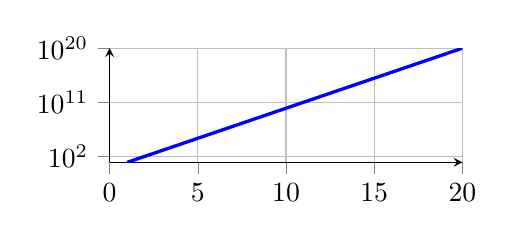
\begin{tikzpicture}
    \begin{axis}[xmin=0,xmax=20,width=0.5\linewidth,height=0.25\linewidth,grid=both,axis x line=left ,axis y line=left, tick align=outside,ymode=log]
      \addplot+[very thick,mark=none,smooth,domain=1:20,samples=20] (\x,{10^(\x)});
    \end{axis}
  \end{tikzpicture}
\end{center}
\item Method based on \emph{nearest neighbors} fail (with Euclidean distance)
\item Hughes phenomenon  \cite{hughes}: 
\begin{quote}
"\emph{With a fixed  design pattern sample, recognition  accuracy can first
increase as the number of  measurements made on a pattern increases,
but  decay  with measurement  complexity  higher  than some  optimum
value.}"
\end{quote}
\item Ill-posed problem:
\begin{itemize}
\item Matrix inversion,
\item Determinant,
\item Overfitting \ldots{}
\end{itemize}
\end{itemize}
\end{frame}
\section{Questions}
\label{sec:org183d6e5}
\begin{frame}[label={sec:org4148527}]{Is there a fake ?}
\begin{onlyenv}<1>
\begin{center}
\includegraphics[width=0.9\linewidth]{./figures/demo.pdf}
\end{center}
\end{onlyenv}

\begin{onlyenv}<2>
\begin{center}
\includegraphics[width=0.9\linewidth]{./figures/demo_1.pdf}
\end{center}
\end{onlyenv}

\begin{onlyenv}<3>
\begin{center}
\includegraphics[width=0.9\linewidth]{./figures/demo_2.pdf}
\end{center}
\end{onlyenv}

\begin{onlyenv}<4>
\begin{center}
\includegraphics[width=0.9\linewidth]{./figures/demo_3.pdf}
\end{center}
\end{onlyenv}

\begin{onlyenv}<5>
\begin{center}
\includegraphics[width=0.9\linewidth]{./figures/demo_4.pdf}
\end{center}
\end{onlyenv}

\begin{onlyenv}<6>
\begin{center}
\includegraphics[width=0.9\linewidth]{./figures/demo_5.pdf}
\end{center}
\end{onlyenv}
\end{frame}

\begin{frame}[label={sec:org5f8ace1}]{Spectra}
\pgfplotstableread{figures/cotton_spectra.txt}\loadedtable
\begin{center}
\begin{tikzpicture}\begin{axis}[xlabel=$\lambda$, ylabel=Reflectance,  xmin=0.4, xmax=2.5, ymin=0,   ymax=1, grid=both,width=0.9\textwidth, height=0.4\textwidth]
    \addplot[smooth,thick] table[x=wavelength,y=dry] from \loadedtable;
    \addplot[smooth,thick,red] table[x=wavelength,y=wet] from \loadedtable;
    \addplot[smooth,thick,blue] table[x=wavelength,y=acid] from \loadedtable;
    \addplot[smooth,thick,orange] table[x=wavelength,y=apple] from \loadedtable;
    \legend{a,b,c,d};
  \end{axis}
\end{tikzpicture}
\end{center}

There are two spectra of the same material (cotton), before and after drying. Which are they ?
\end{frame}

\begin{frame}[label={sec:org7a4b31c}]{Gaussian distribution}
What is the number of parameters to estimate for a Gaussian distribution

\begin{itemize}
\item <2-> The mean: \(d\)
\item <3-> The covariance matrix: \(d(d+1)/2\)
\end{itemize}

\begin{block}<4->{Total: \(d(d+3)/2 \approx d^2/2\)}
\begin{center}
  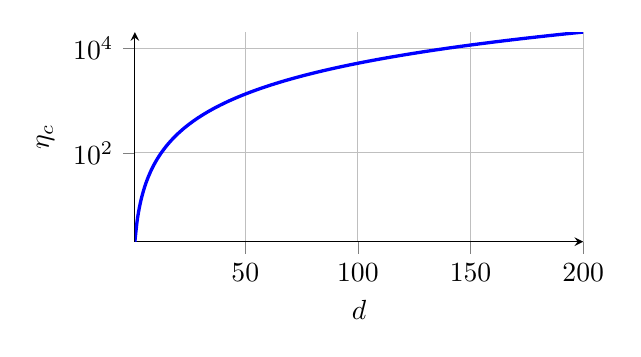
\begin{tikzpicture}
    \begin{axis}[ymode=log,xmin=1,xmax=200,width=0.6\linewidth,height=0.35\linewidth,grid=both,axis x line=left ,axis y line=left, tick align=outside,xlabel = $d$,ylabel = $\eta_c$]
      \addplot+[very thick,mark=none,smooth,domain=1:200,samples=200] (\x,{\x*(\x+3)/2});
    \end{axis}
  \end{tikzpicture}
\end{center}
\end{block}
\end{frame}
\section{References}
\label{sec:org4da3679}
\begin{frame}[fragile,allowframebreaks,label=]{Bibliography}
\printbibliography
\end{frame}
\end{document}